%%%%%%%%%%%%%%%%%%%%%%%%%%%%%%%%%%%%%%%%%
%
% Optics and Radar -based observations
% Assignment 2
%
%%%%%%%%%%%%%%%%%%%%%%%%%%%%%%%%%%%%%%%%%

%----------------------------------------------------------------------------------------
%	DOCUMENT CONFIGURATIONS
%----------------------------------------------------------------------------------------
%   FINAL VERSION
\documentclass{article}

\title{\textbf {Optics and Radar Based Observations} \\ Assignment 2\\ Pulse Modulation Techniques} % Title

\def\authors{
Ivan \v Sinkarenko\\
Anuraj Rajendraprakash
}
\author{\authors}

\usepackage{graphicx}
\usepackage{fullpage}
\begin{document}

\maketitle % Insert the title, author and date

\centerline{Referee: Dr. Anita Enmark}

%\vspace{10mm}
%\begin{figure}[h!]
%\centering
%\centerline{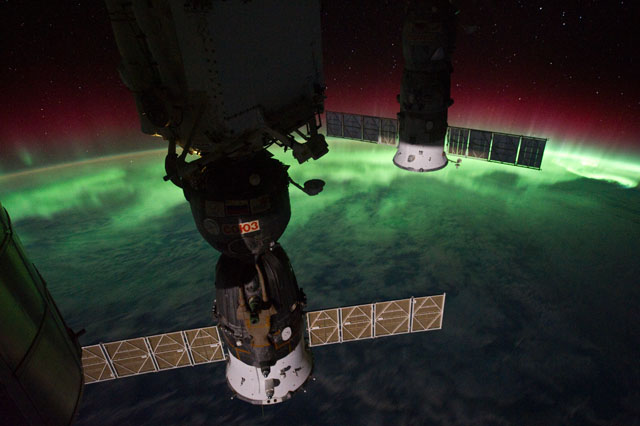
\includegraphics[width=\textwidth]{Figures/iss.jpg}}
%\label{fig:iss}
%\end{figure}

\setlength\parindent{0pt} % Removes all indentation from paragraphs

\renewcommand{\labelenumi}{\alph{enumi}.} % Make numbering in the enumerate environment by letter rather than number (e.g. section 6)
\clearpage

\tableofcontents

\listoffigures

\clearpage

%----------------------------------------------------------------------------------------
%	SECTION 1. Introduction
%----------------------------------------------------------------------------------------

\section{Introduction}
Polar lights, also known as Aurora Polaris, is the collective term for the aurora seen over the northern and southern poles of the Earth. They are referred to as northern lights (Aurora Borealis) and southern lights (Aurora Australis). Research of the polar lights has been carried out for many decades; there are many theories about how this spectacular display is created. \cite{Stenberg:2012ab}\\ 
The primary objective of this practical was to understand the phenomena of auroras and be able to classify it according to different criteria. As a part of this assignment, it was also required to study and correlate the riometer and magnetometer data during the occurance of auroras.
 
%----------------------------------------------------------------------------------------
%	SECTION 2. Part 1
%----------------------------------------------------------------------------------------

\section{Part 1}


%----------------------------------------------------------------------------------------
%	SECTION 3. Part 2
%----------------------------------------------------------------------------------------

\section{Part 2}

%----------------------------------------------------------------------------------------
%	SUBSECTION 3.1. Part 2A
%----------------------------------------------------------------------------------------

\subsection{Part 2A}

%----------------------------------------------------------------------------------------
%	SUBSECTION 3.2. Part 2B
%----------------------------------------------------------------------------------------

\subsection{Part 2B}

%----------------------------------------------------------------------------------------
%	SECTION 4. REFERENCES
%----------------------------------------------------------------------------------------

\begin{thebibliography}{9}

\bibitem{Stenberg:2012ab}
Stenberg, G.  (2012).
\newblock {\em Practical 1. Aurora Borealis}.
\newblock Swedish Institute of Space Physics, Kiruna, Sweden.

\bibitem{KivelsonRussell:1996isp}
Kivelson M. ~G. and Russell C. ~T.  (1996).
\newblock {\em Introduction to Space Physics}.
\newblock Cambridge University Press, Melbourne, Australia.

\end{thebibliography}

%----------------------------------------------------------------------------------------
%	SECTION 5. Appendix 2A
%----------------------------------------------------------------------------------------

\section{Appendix 2A. Matlab code of Part 2A}

%----------------------------------------------------------------------------------------
%	SECTION 6. Appendix 2B
%----------------------------------------------------------------------------------------

\section{Appendix 2B. Matlab code of Part 2B}

%----------------------------------------------------------------------------------------
%	SECTION 7. Confirmation
%----------------------------------------------------------------------------------------

\section{Acknowledgements}


\end{document}